\subsection{A Simple Lane Change}
\begin{itemize}
	\item We first present this scenario in \cite{blah}
	\item Other authors \cite{blah} have considered with static obstacles
	\item Counterexamples are somewhat obvious
	\item Inductive invariance argument allows verification of infinite time properties
	\item Most examples involving forward safety are monotonic ie selecting a lower operating speed implies an decrease in stopping time and improves the forward safety of the vehicle. 
	\item In such problems there are no ``holes" in the interval. 
	\item Resulting proofs seem to indicate that testing would be sufficient to find counterexamples because unsafe results occur at extreme points in the state space only.
	\begin{itemize}
		\item Verification still provides a guarantee of safety that was not previously available. 
		\item Verification is still useful for formally verifying specifications and interaction between supplier systems and vehicle dynamics.
		\item Helps to search for viable combinations of specifications
	\end{itemize}
	\item We extend this scenario with differential inclusions. 
	\item Problem: we are forced into the tree representation because we cannot bring the trajectory generator in the dReach framework, requires external libraries and iteration. Could be remedied via creation of a lookup table or Neural Network. Alternative is to change the trajectory generation strategy such as Pure Pursuit.
\end{itemize}

Define the behavioral controller as a hybrid system. Fig \ref{fig:lc} details the behavioral controller for the lane changing scenarios. 
\begin{figure}[h]
	\centering
	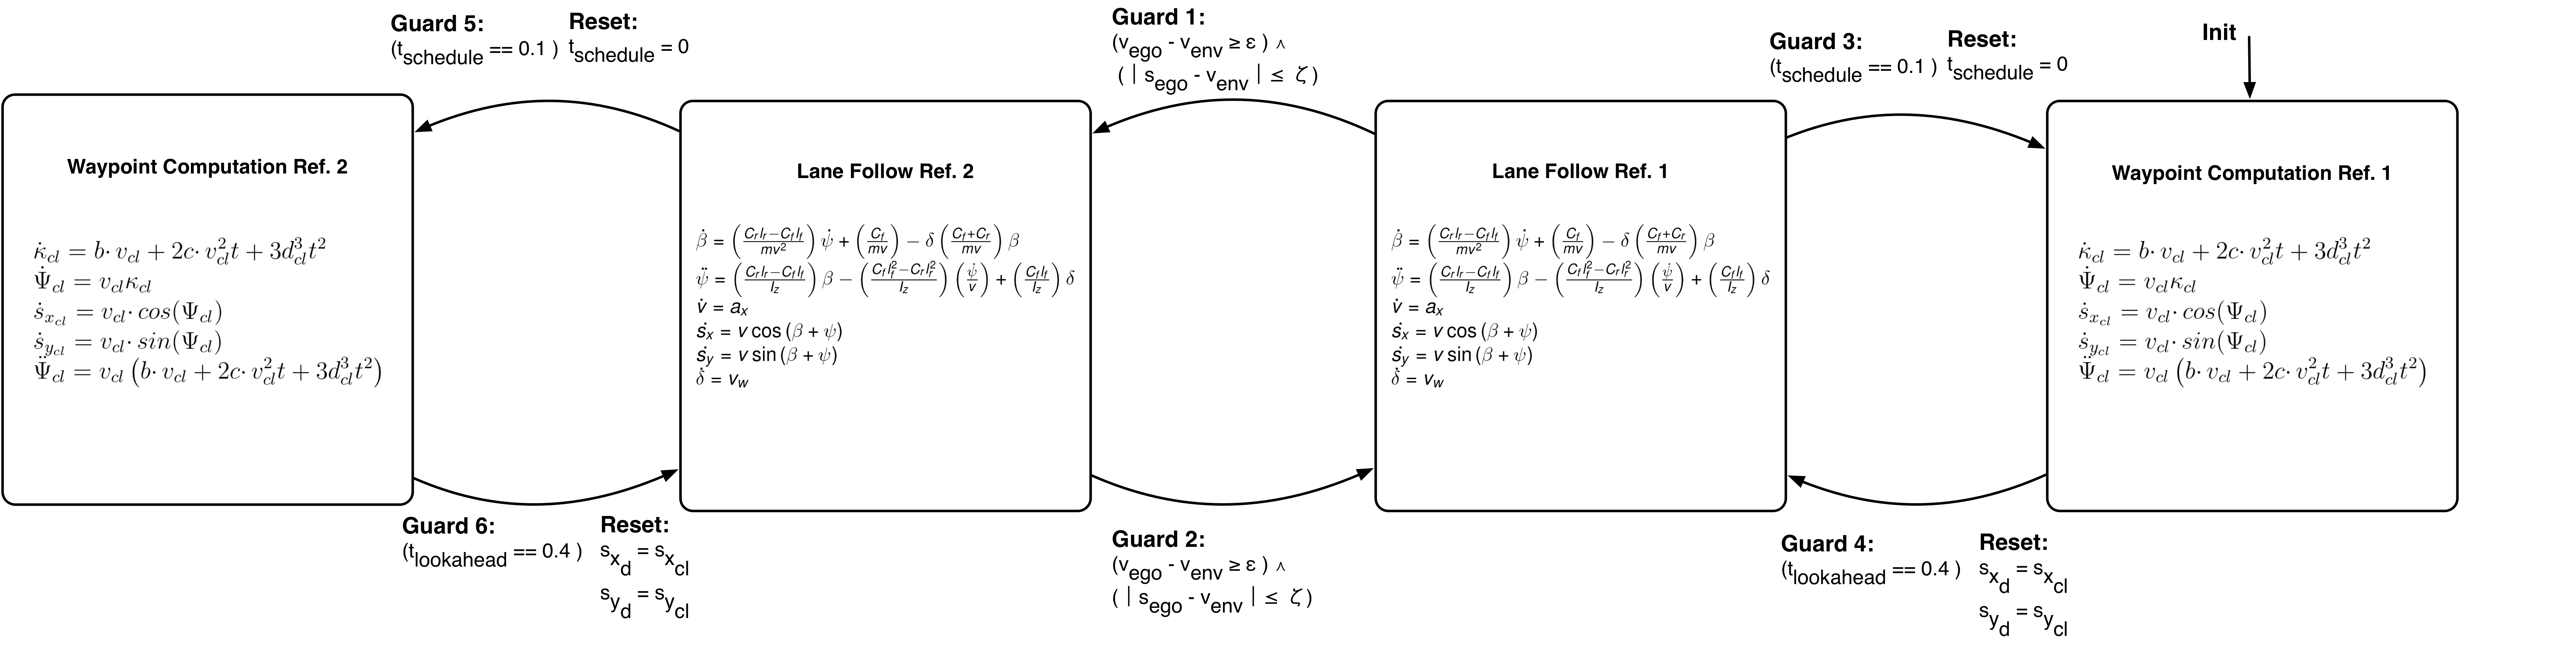
\includegraphics[width=\textwidth]{figures/arch-ego-automaton}
	\caption{The behavioral controller governing the lane selection of the ego-vehicle}
	\label{fig:lc}
\end{figure}

\subsection{Variations in Road Geometry}
%\textbf{Random Ideas, not to be taken seriously}
%\begin{itemize}
%	\item Can we think of a type theoretic description of configuration space rather than set theoretic?
%	\item For example think of configuration space as a type
%	\item Pose and Goal can then be considered points of the configuration space type 
%	\item There exists many paths between a single pose and goal pair, all of these paths are equivalent from a type theoretic perspective.
%\item Narrow down an instance of these paths by describing a decision procedure necessary to generate the path ie pure pursuit or cubic splines, the type of these functions is a path between goal and pose. 
%\end{itemize}

\begin{itemize}
	\item In order to pursue more complex scenarios with more expressive agents we propose a variation in the trajectory generation strategy which admits a closed form
	\item Implement pure pursuit trajectory generation strategy...
\end{itemize}
\begin{itemize}
	
	\item Open question if we can guarantee infinite time properties in general case, or on road by road basis via inductive invariant. 
	\item A second question of interest is the scalability of results involving multiple agents and curved roads. 
	\item Pure Pursuit can be represented directly in the Hybrid Program and admits a closed form solution for curvature.
	\item Using a Hybrid program we now show how the number of paths through the state space grows exponentially with the addition of other agents and events as well as increases in search depth. 
\end{itemize}

We present a scenario as shown in Figure \ref{fig:scenario2}
\begin{figure}
	\centering
	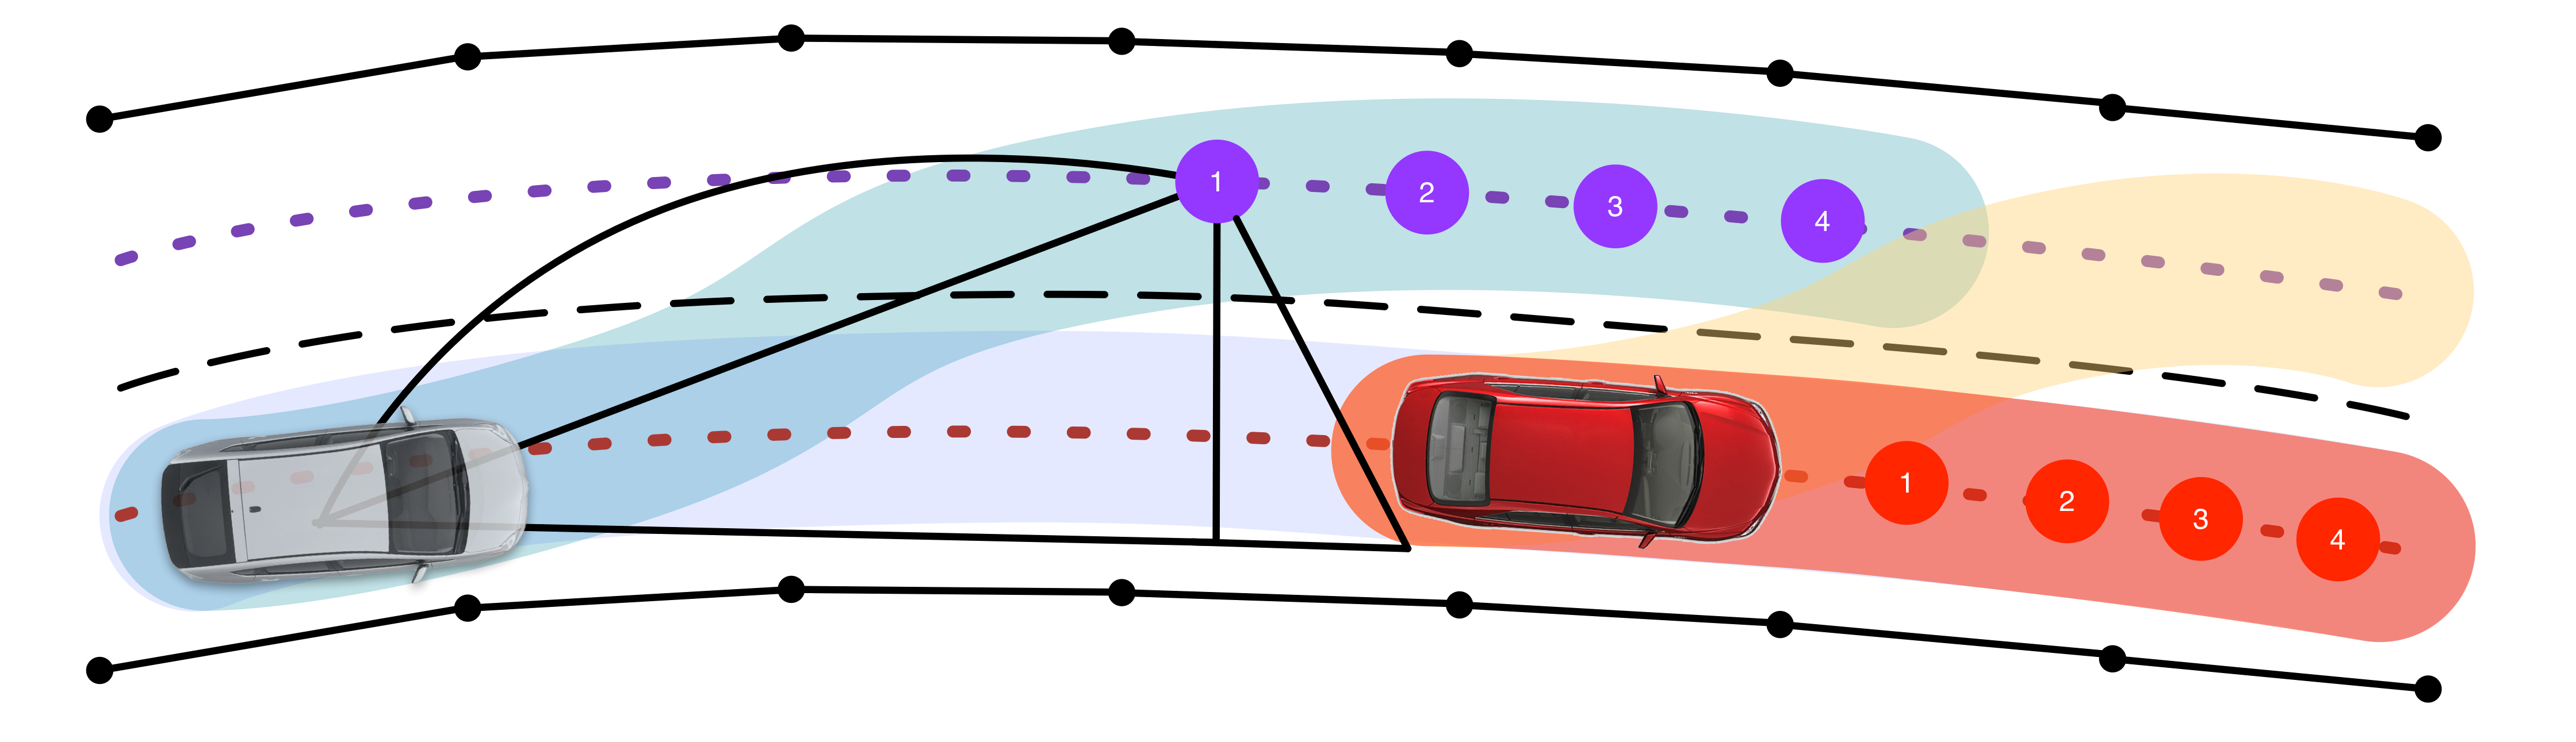
\includegraphics[scale=.4]{figures/scenario2}
	\caption{A graphical representation of the lane change scenario on a curved road}
\end{figure}
\begin{itemize}
	\item The previous example is the simplest possible instantiation of a lane change scenario
	\item Here we present an increasingly nuanced view of the the vehicle environment system
	\begin{itemize}
		\item Singleton inital sets and deterministic transitions
		\item Initial sets defined by intervals
		\item Non-determinism as applied to discrete decisions by the environment
		\item Automaton complexity in terms of states as number of agents grows
		\item Automaton complexity in terms of states as number of reference trajectories grows
		\item Search complexity in terms of path length as number of agents grows
		\item Search complexity in terms of path length as number of reference trajectories grows
		\item Non-deterministic scheduling of trajectory update
		\item Environment agents continuous dynamics are represented as differential inclusions (another form of non-determinism)
		\item Ego vehicle agents continuous dynamics are disturbed via errors represented as differntial inclusions
		\item Ego vehicle and environmental agents subjected to discrete events representing sensor or actuator failures.
	\end{itemize}
\end{itemize}

\subsection{Intersection}
Fig \ref{fig:intersection} details the behavioral controller for the intersection scenario. 

\begin{figure}
	\centering
	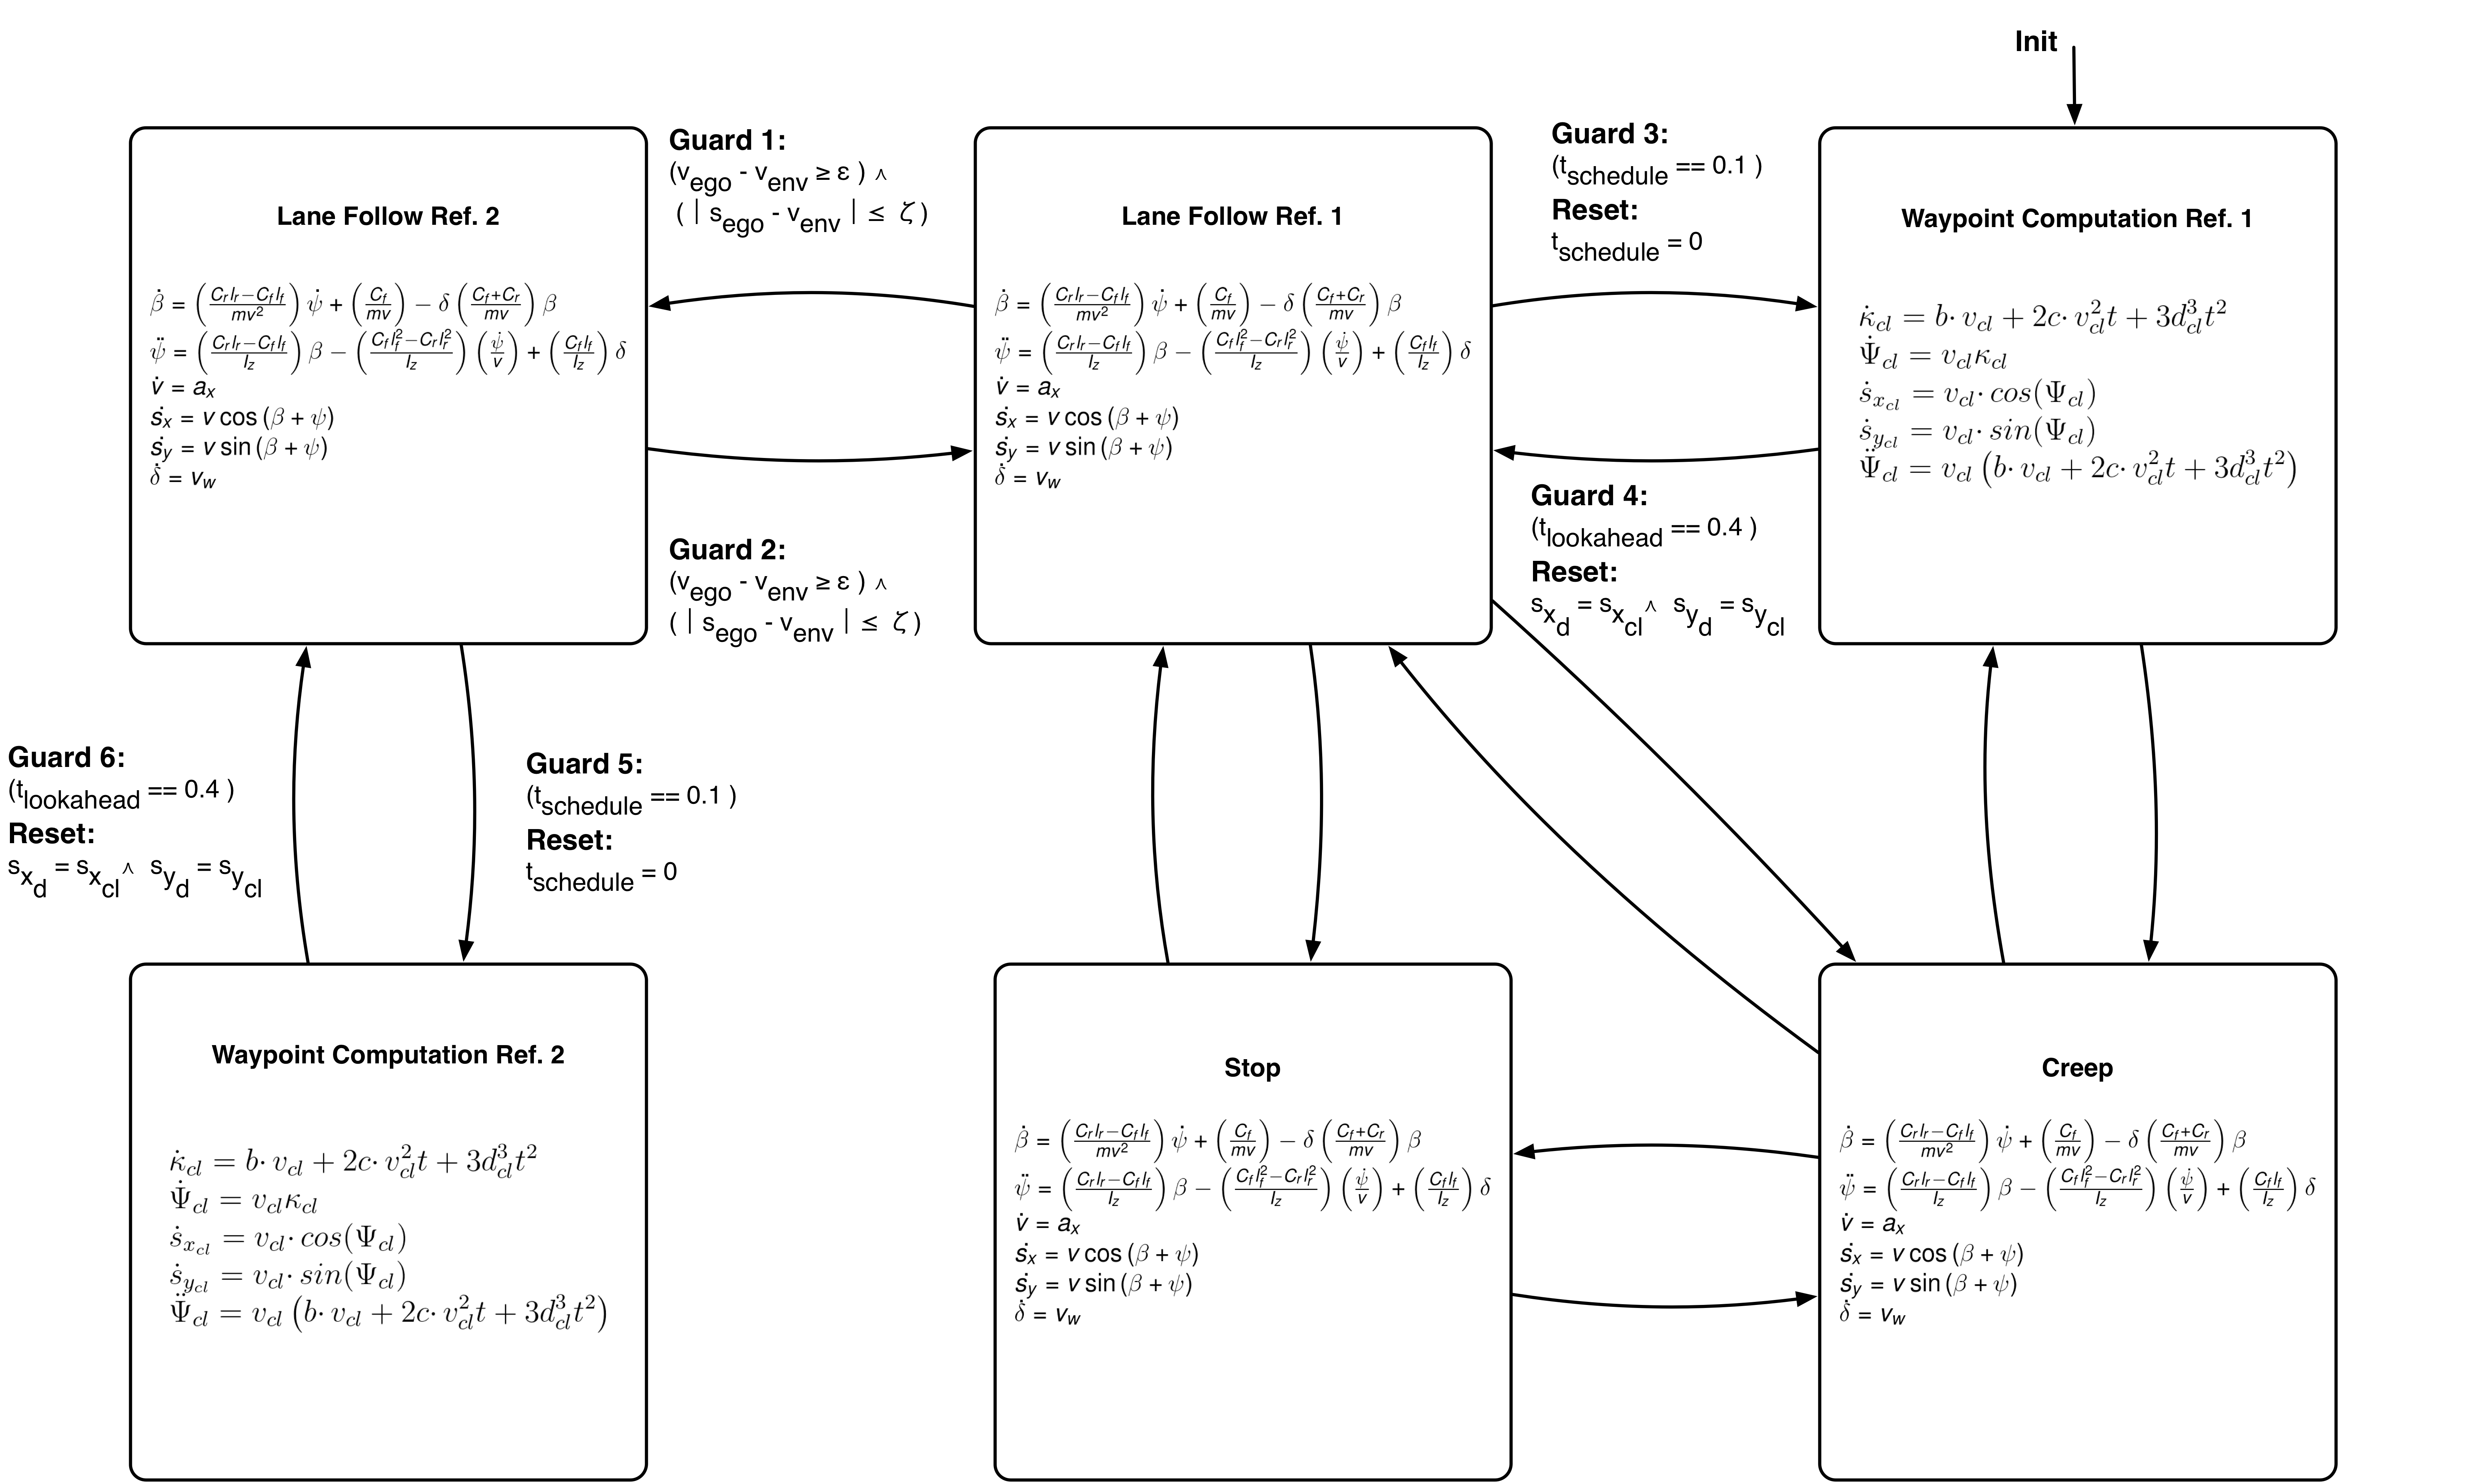
\includegraphics[width=\textwidth]{figures/intersection}
	\caption{Composed Hybrid Automaton for Intersection Scenario}
	\label{fig:intersection}
\end{figure}
